\documentclass[A4]{report}
\usepackage[francais]{babel}
\usepackage[utf8]{inputenc}

% pour les algos
\usepackage{algorithm, algorithmic}
\floatname{algorithm}{Algorithme}
\renewcommand{\algorithmicrequire}{\textbf{Précondition:}}
\renewcommand{\algorithmicensure}{\textbf{Postcondition:}}
\renewcommand{\algorithmicend}{\textbf{fin}}
\renewcommand{\algorithmicif}{\textbf{si}}
\renewcommand{\algorithmicthen}{\textbf{alors}}
\renewcommand{\algorithmicelse}{\textbf{sinon}}
\renewcommand{\algorithmicfor}{\textbf{pour}}
\renewcommand{\algorithmicforall}{\textbf{pour chaque}}
\renewcommand{\algorithmicdo}{\textbf{:}}
\renewcommand{\algorithmicwhile}{\textbf{tant que}}
\renewcommand{\algorithmicloop}{\textbf{boucle}}
\renewcommand{\algorithmicrepeat}{\textbf{répéter}}
\renewcommand{\algorithmicuntil}{\textbf{jusqu'à}}

% pour les tableaux
\usepackage{array}
\usepackage{multirow}
\usepackage{booktabs}

% pour les maths
\usepackage{amssymb,amsmath}
\usepackage{amsthm}
\newtheorem{thm}{Théorème}[chapter]
\newtheorem{cor}[thm]{Corollaire}
\newtheorem{lem}[thm]{Lemme}
\theoremstyle{remark}
\newtheorem*{rmk}{Remarque}
% gestion des marges
\usepackage[left=4cm,right=3cm,top=2cm,bottom=2cm]{geometry}

% Definition du petit header visible sur les pages non plain
\usepackage{fancyhdr}
\pagestyle{fancy}
\renewcommand{\chaptermark}[1]{\markright{\thechapter\ #1}}
\renewcommand{\sectionmark}[1]{\markright{\thesection\ #1}}
\fancyhead[R]{\thepage}
\fancyhead[C]{\scshape\rightmark}
\fancyhead[L]{}
\fancyfoot[C]{}
\renewcommand{\headrulewidth}{0pt}

% pour les bouts de code
\usepackage{listings}
\lstset{language=C,
		  tabsize=2,
		  numberstyle=\tiny,
		  basicstyle=\ttfamily\small,
		  commentstyle=\ttfamily\small,
		  numbersep=5pt}
\usepackage{fancyvrb}

% Pour les n'images
\usepackage[pdftex]{graphicx,color}

% Page de garde à refaire avec chtite n'images et noms de tout le monde
\title{Sujet 1 : Algorithme d'ordonnancement}
\author{Groupe 1}
\date{Année 2006-2007}


\newcommand{\sups}[1]{\raisebox{1ex}{\small #1}}

\begin{document}
\begin{titlepage}
\begin{center}
{\large
Ministère de l'Education Nationale \\
\vspace{0.8cm}
Université Montpellier II \\
\vspace{1.5cm}
Rapport de projet de l'unité d'enseignement ULIN507 \\
de la licence informatique 3\sups{ème} année \\
effectué lors du second semestre de l'année 2006-2007 \\
}
\vspace{4cm}
{\huge Sujet 1 }\\
\vspace{0.2cm}
\hrule
\vspace{0.2cm}
{\Huge Algorithmes d'ordonnancement}
\vspace{7cm}
\end{center}
\begin{flushright}
{\raggedleft
\begin{tabular}{r|l}
Auteurs & ABERMAN Jonathan \\
& BOZADJIEV Victor \\
& DUBUISSON Nathalie \\
& JACINTO Jean-Pierre \\
& MENDES Samuel \\
& MICHEL Kevin \\
& PANCALDI Vincent \\
& PERALTA Emmanuel \\
& RAFFIN Jonathan \\
& RENGOT Thomas \\
& ROUS Guillaume \\
\end{tabular}
}
\end{flushright}
\end{titlepage}
\tableofcontents

\chapter{Introduction}
\section{Problématique de l'ordonnancement}
Le sujet ici présenté est l'étude de plusieurs problèmes relatifs à
l'ordonnancement de tâches, c'est à dire la répartition et la permutation de
l'ordre d'un ensemble de tâches sur une ou plusieurs machines avec diverses
contraintes à satisfaire. Certaines contraintes étant strictes (dépendances entre
certaines tâches, nombre de machines ...), d'autres étant plus flexibles et nous servant d'objectif à
optimiser (durée totale d'exécution principalement).

Parmi les problèmes
présentés, certains sont solubles en temps polynomial et dans ce cas une
solution optimale est proposée, d'autres obligent par contre à employer des heuristiques polynomiales afin de conserver des temps de calcul raisonnables. Ces heuristiques ont cependant toutes une borne supérieure d'efficacité au moins inférieure au double de la solution optimale.

\section{Objectifs du projet}
Notre objectif tout d'abord est d'étudier ces problèmes, de leur trouver une
solution, de démontrer son optimalité ou sa borne maximale d'optimalité et enfin
la complexité de son implémentation. La seconde étape est l'implémentation
pratique de ces algorithmes et enfin une interface permettant de les tester et
de visualiser leur performance.

\chapter{Démonstrations des algorithmes}
\section{Répartition de tâches sans précédences sur plusieurs machines}
\subsection{Problème}
Dans ce problème, il s'agit de répartir un ensemble de tâches de durées 
diverses, sans dépendances entre elles sur plusieurs machines identiques, 
l'objectif de l'ordonnancement étant de minimiser le temps total de calcul.
Nous allons tout d'abord utiliser une répartition de type premier arrivé-premier 
servi sur l'ensemble des tâches, puis utiliser l'algorithme de coffman-graham en 
utilisant la durée des tâches comme relation d'ordre de priorité avant de les 
répartir.

\subsection{Algorithme naïf}
\subsubsection{Présentation}
Le principe est de prendre une liste de tâches dans un ordre quelconque et 
à chaque itération de prendre la première tâche de la liste et de l'affecter 
à la première machine disponible.
\subsubsection{Exemple}
Prenons ${n=13}$ ${m=4}$ et ${(p_{1},p_{2},...,p_{12},p_{13}) 
= (1,1,...,1,4)}$.\\
L'application de l'algorithme à cet ensemble donne le résultat suivant, ayant 
pour temps d'exécution total $7$ :
\begin{center}
$m_{1} = {p_{1},p_{5},p_{9},p_{13}}$ \\
$m_{2} = {p_{2},p_{6},p_{10}}$ \\
$m_{3} = {p_{3},p_{7},p_{11}}$ \\
$m_{4} = {p_{4},p_{8},p_{12}}$ \\
\end{center}
Or on peut facilement produire à la main un meilleur résultat :
\begin{center}
$m_{1} = {p_{1},p_{4},p_{7},p_{10}}$ \\
$m_{2} = {p_{2},p_{5},p_{8},p_{11}}$ \\
$m_{3} = {p_{3},p_{6},p_{9},p_{12}}$ \\
$m_{4} = {p_{13}}$ \\
\end{center}
Celui-ci a un temps d'exécution total de $4$, les bornes inférieures que nous 
allons donner par la suite pour $C^*_{max}$ montrent que c'est un résultat 
optimal.
\subsubsection{Mesure du ratio de performance}
Commençons tout d'abord par poser deux bornes inférieures pour $C^*_{max}$, 
toutes deux relativement triviales. La première est déterminée par le cas 
optimal où toutes les machines sont occupées pendant toute la durée du calcul, 
et donc où toutes les machines s'arrètent de travailler en même temps.
\begin{equation}
\label{graham-chien}
C^*_{max} \geq \frac{\sum_{i=1}^n p_{i}}{m}
\end{equation}
Une seconde borne encore plus triviale est la durée de la plus longue de toutes 
les tâches.
\begin{equation}
\label{graham-lapin}
C^*_{max} \geq max^n_{i=1}(p_{i})
\end{equation}
Soit $j'$ la tâche qui se termine à $C^{LS}_{max}$ :
\begin{equation}
C^{LS}_{max} = t_{j'} + p_{j'}
\end{equation}
Nous avons de plus :
\begin{equation}
p_{j'} \leq max^n_{i=1}(p_{i})
\end{equation}
Ce qui combiné avec \eqref{graham-lapin} nous donne le résultat suivant :
\begin{align}
p_{j'} &\leq C^*_{max} \\
\label{graham-canard}
C^{LS}_{max} &\leq t_{j'} + C^*_{max}
\end{align}
Or $t_{j'}$ est le moment ou $j'$ débute, ce qui signifie que lors de son 
affectation à une machine toute les autres machines sont déja occupées jusqu'à 
au moins $t_{j'}$ ce qui signifie qu'à cet instant les machines ont déja calculé 
pendant une durée de $m*t_{j'}$, or le temps de travail des machines est 
forcément inférieur à la durée totale de calcul des tâches, ce qui nous donne :
\begin{align}
m*t_{j'} &\leq \sum_{i=1}^n p_{i} \\
\label{graham-ours}
t_{j'} &\leq \frac{\sum_{i=1}^n p_{i}}{m} \\
t_{j'} &\leq C^*_{max}
\end{align}
Ce qui combiné avec \eqref{graham-canard} nous donne enfin le ratio de 
performance :
\begin{align}
C^{LS}_{max} &\leq 2*C^*_{max} \\
\frac{C^{LS}_{max}}{C^*_{max}} &\leq 2 
\end{align}
\subsubsection{Complexité de l'implémentation}
Pour implémenter cet algorithme, nous avons besoin de deux structures de 
données, la première est la liste des tâches, étant donné que nous ne voulons 
que prendre le premier élément, une pile ou une itération sur un tableau sont 
suffisantes. La seconde structure est celle qui permet de savoir à chaque 
itération sur un élément de la liste des tâches quelle est la première machine 
disponible, nous avons choisit pour cela un tas binaire ordonné avec la première 
machine disponible en haut du tas.

Le tas binaire permet d'accéder à cet élément en temps constant, de le supprimer 
en $O(log(m))$ et de le réinserer une fois la durée de la nouvelle tâche ajoutée 
en $O(log(m))$.
L'opération complète que l'on nomme $Augmenter\_minimum(tas, duree)$ prend donc 
$O(log(m))$ et est répétée pour chaque tâche, ce qui nous fait une complexité 
totale de $O(n.log(m))$.

On note enfin que la création du tas initial avec toute les durées à 0 et avec 
un élément pour chaque machine se fait en $O(m)$ avec une implémentation en 
tableau du tas, $m$ étant typiquement inférieur à $n$ (sans quoi 
l'ordonnancement est trivial) cela n'influence pas la complexité.
\begin{algorithm}
\caption{Augmenter\_minimum(tas, duree)}
\begin{algorithmic}
\STATE $elem \leftarrow extraire\_minimum(tas)$
\STATE $machine \leftarrow machine(elem)$
\STATE $duree(elem) \leftarrow duree(elem) + duree$
\STATE $inserer(tas, elem)$
\STATE \textbf{retourner} $machine$
\end{algorithmic}
\end{algorithm}

\begin{algorithm}
\caption{Ordonnancement\_LS(taches)}
\begin{algorithmic}
\STATE $tas = creer\_tas()$
\FORALL{$tache$ \textbf{dans} $taches$}
\STATE $machine(tache) = Augmenter\_minimum(tas, duree(tache))$
\ENDFOR
\end{algorithmic}
\end{algorithm}
\subsection{Algorithme de Coffman-Graham}

\subsubsection{Présentation}
L'algorithme de Coffman-Graham est similaire au précédent, avec pour seul 
différence un tri préalable des tâches selon la durée, et ceci de manière 
décroissante. Le tri induit un calcul préalable de complexité $O(n.log(n))$ mais 
améliore, comme nous allons le démontrer le ratio de performance en l'abaissant 
à $\frac{4}{3}$.
\begin{algorithm}
\caption{Ordonnancement\_LPT(taches)}
\begin{algorithmic}
\STATE $Trier(taches, duree(b)-duree(a))$
\STATE $Ordonnancement\_LS(taches)$
\end{algorithmic}
\end{algorithm}
\subsubsection{Démonstration}
Nous pouvons tout d'abord partir de l'équation \eqref{graham-ours} trouvée lors 
de l'étude de $C^{LS}_{max}$ :
\begin{align}
C^{LPT}_{max} &= t_{j'} + p_{j'} \\
C^{LPT}_{max} &\leq \frac{\sum_{i=1}^n p_{i}}{m} + p_{j'} \\
\end{align}
Puis en employant \eqref{graham-chien}, nous obtenons :
\begin{equation}
C^{LPT}_{max} \leq C^*_{max} + p_{j'}
\end{equation}
Distinguons maintenant deux cas, selon la valeur de $p_{j'}$, tout d'abord si 
$p_{j'} \leq \frac{C^*_{max}}{3}$ :
\begin{align}
C^{LPT}_{max} &\leq C^*_{max} + \frac{C^*_{max}}{3} \\
C^{LPT}_{max} &\leq \frac{4}{3} C^*_{max} \\
\frac{C^{LPT}_{max}}{C^*_{max}} &\leq \frac{4}{3}
\end{align}
Cependant si $p_{j'} > \frac{C^*_{max}}{3}$ la solution n'est pas aussi simple.  
Tout d'abord on peut écarter le cas où $n\leq m$, dans ce cas on ne peut faire 
mieux que de mettre zéro ou une tâche sur chaque machine, la solution est 
triviale. Étudions maintenant le cas contraire.

Appelons $M$ la machine traitant $j'$, celle-ci traite un certain nombre 
d'autres tâches. On sait que le temps d'exécution de $M$ est le plus élevé de 
toutes les machines et détermine $C^{LPT}_{max}$. On sait aussi que les autres 
machines ont toutes un temps d'exécution d'au moins $t_{j'}$. On sait enfin que  
toutes les tâches sur $M$ sont de durées supérieures à $p_{j'}$ étant donné que 
$j'$ est la dernière traitée et que les tâches sont traitées par durée 
décroissante.

On ne peut enlever une tâche de $M$ pour la mettre sur une autre machine, les 
autres machines ayant un temps d'exécution déjà supérieur à $t_{j'}$ et les 
tâches de $M$ ayant toutes une durée supérieure à $p_{j'}$, le temps d'exécution 
de l'autre machine deviendrait supérieur à $t_{j'}+p_{j'}$ donc supérieur 
à $C^{LPT}_{max}$ ce qui ne raccourcirait pas l'ordonnancement.

Cela signifie donc que pour réduire la durée d'exécution de $M$, il faut 
permuter des tâches de $M$ avec celles d'autres machines. Si on permute une 
tâche $a$ de $M$ avec une tâche $b$ d'une autre machine, la tâche $b$ se doit 
d'être de durée supérieure à $p_{j'}$ sinon cela signifie qu'elle démarre 
après $t_{j'}$ et donc que la machine $M'$ d'où vient $b$ aura un temps 
d'exécution supérieur à $t_{j'}+p_{j'}$ ce qui ne raccourcirait toujours pas 
l'ordonnancement.

Enfin on remarque que s'il y a trois tâches ou plus avant $j'$ sur $M$, alors 
$t_{j'} > 3*p_{j'}$. Or $C^*_{max} \geq \frac{\sum_{i=1}^n p_{i}}{m} \geq 
t_{j'}$, ce qui nous amène enfin à $C^*_{max} \geq 3*p_{j'}$ ce qui contredit 
notre hypothèse sur $p_{j'}$.  Il y a donc au plus deux tâches avant $j'$ sur 
$M$.

Cela signifie donc que l'on peut avoir au plus deux permutations pour réduire la 
durée d'exécution de $M$ et qu'on l'on ne peut répartir l'excédent que sur au 
plus deux autres machines. Étant donné que toutes les autres machines ont un 
temps d'exécution supérieur à $t_{j'}$ on ne peut pas réduire la durée de $M$ de 
plus de $\frac{2}{3}p_{j'}$. Ce qui nous amène à la conclusion :

\begin{align}
C^*_{max} &\geq C^{LPT}_{max} - \frac{2*p_{j'}}{3} \\
C^*_{max} &\geq C^{LPT}_{max} - \frac{2*C^*_{max}}{9} \\
\frac{11}{9}C^*_{max} &\geq C^{LPT}_{max} \\
\frac{12}{9}C^*_{max} &\geq C^{LPT}_{max} \\
\frac{4}{3} &\geq \frac{C^{LPT}_{max}}{C^*_{max}} \\
\end{align}

Nous avons ainsi démontré que le ration de performance de $C^{LPT}_{max}$ est 
inférieur à $\frac{4}{3}$ dans tout les cas, CQFD.

\section{Ordonnancement de tâches à priorité pondérées}
\subsection{Problème}
Il s'agit ici d'ordonnancer un ensemble de {\em n} tâches sur une seule machine.
Comme dans les problème précédent on considère qu'elles ne sont pas
interdépendantes. En revanche, cette fois-ci on considère avec la durée un poids
associé pour chaques tâches. Il nous faut donc une solution tenant compte de ces
deux propriétés dans l'ordre de priorité. 
 
\subsection{Principe}
La règle de Smith, ou du Temps Opératoire Minimum Pondéré est un moyen 
d'ordonnancer des tâches en donnant priorité aux tâches ayant le plus faible 
quotient de leur durée opératoire à leur coefficient de pondération. Wayne Smith 
a démontré en 1956 que cette règle produit une séquence optimale sur une machine 
lorsque toutes les tâches sont disponibles simultanément.\\
L'algorithme est très simple, il suffit de trier les tâches selon le quotient 
susmentionné, ceci se fait bien évidemment en $O(n.log(n))$.

\subsection{Algorithme}
\begin{algorithm}
\caption{Algorithme de la règle de Smith}
\begin{algorithmic}
\STATE $Trier(taches, (p_i*w_j - p_j*w_i))$
\end{algorithmic}
\end{algorithm}

\subsection{Exemple}
Nous voulons ordonner $n = 6$ tâches tel que :
\begin{center}
\begin{tabular}{|c|c|c|c|c|c|c|}
\hline
$j$ & 1 & 2 & 3 & 4 & 5 & 6  \\
\hline
$p_j$ & 8 & 6 & 3 & 7 & 4 & 8  \\
$w_j$ & 8 & 3 & 6 & 7 & 8 & 1  \\
\hline
$\frac{p_j}{w_j}$ & 1 & 2 & $\frac{1}{2}$ & 1 & $\frac{1}{2}$ & 8 \\
\hline
\end{tabular}
\end{center}
En triant les tâches nous obtenons $j_3,j_5,j_1,j_4,j_2,j_6$.

\subsection{Démonstration}
Étant donnée une suite $S$ de $n$ tâches $J^S_1...J^S_n$ de temps d'exécution 
$p^S_1...p^S_n$ et munies de poids $w^S_1...w^S_n$ strictement positifs.  On dit 
que celle-ci respecte la règle de Smith si elle respecte la relation d'ordre:
\begin{equation}
\forall i \in [1,n-1]: \quad \frac{p^S_i}{w^S_i} \leq 
\frac{p^S_{i+1}}{w^S_{i+1}}
\end{equation}
Que l'on peut étendre par transitivité :
\begin{equation}
\forall i,j \in [1,n-1]: \quad i\leq j \Leftrightarrow \frac{p^S_i}{w^S_i} \leq 
\frac{p^S_j}{w^S_j}
\end{equation}
Et enfin que l'on peut aussi écrire :
\begin{equation}\label{inek}
\forall i,j \in [1,n-1]: \quad i\leq j \Leftrightarrow p^S_iw^S_j \leq 
p^S_jw^S_i
\end{equation}

\begin{rmk}
La règle de Smith étant une relation d'ordre, si une suite $S$ la respecte, 
alors toute sous-suite de $S$ la respecte.
\end{rmk}

Soit $T(S)$ la valeur du temps opératoire pondéré d'une suite $S$ de longueur 
$n$, calculée ainsi:
\begin{equation}
T(S) = \sum_{i=1}^n \left(w^S_i\sum_{j=1}^i\left(p^S_j\right)\right)
\end{equation}

\subsection{Déplacement d'un élément}
Prenons une suite $L$ de $n$ tâches ordonnées selon la règle de Smith, et une 
permutation $L'$ de $L$ telle que:
\begin{align}
L'_1 &= L_q \\
\forall i\in[2,q]:L'_i &= L_{i-1} \\
\forall i\in[q+1,n]:L'_i &= L_i
\end{align}
C'est à dire la suite $L$ avec son $q$\textsuperscript{ième} élément replacé au 
début.  Afin de comparer $T(L')$ à $T(L)$, développons $T(L')$:
\begin{align}
T(L') &= \sum_{i=1}^n \left(w^{L'}_i\sum_{j=1}^i\left(p^{L'}_j\right)\right) \\
&= w^{L'}_1p^{L'}_1 + \sum_{i=2}^q 
\left(w^{L'}_i\sum_{j=1}^i\left(p^{L'}_j\right)\right) + \sum_{i=q+1}^n
\left(w^{L'}_i\sum_{j=1}^i\left(p^{L'}_j\right)\right) \\
&=  w^{L'}_1p^{L'}_1 + \sum_{i=2}^q 
\left(w^{L'}_i\biggl(p^{L'}_1+\sum_{j=2}^i\left(p^{L'}_j\right)\biggr)\right) 
+ \sum_{i=q+1}^n
\left(w^{L'}_i\sum_{j=1}^i\left(p^{L'}_j\right)\right) \\
&= w^{L'}_1p^{L'}_1 + \sum_{i=2}^q \left(w^{L'}_ip^{L'}_1\right) +  \sum_{i=2}^q 
\left(w^{L'}_i\sum_{j=2}^i\left(p^{L'}_j\right)\right) + \sum_{i=q+1}^n
\left(w^{L'}_i\sum_{j=1}^i\left(p^{L'}_j\right)\right)
\end{align}
Maintenant, remplaçons les éléments de $L'$ par des éléments de $L$:
\begin{align}
T(L') &=  w^{L}_qp^{L}_q + \sum_{i=1}^{q-1} \left(w^{L}_ip^{L}_q\right) 
+  \sum_{i=2}^q \left(w^{L}_{i-1}\sum_{j=2}^i\left(p^{L}_{j-1}\right)\right) 
+ \sum_{i=q+1}^n \left(w^{L}_i\sum_{j=1}^i\left(p^{L}_j\right)\right)\\
&= \sum_{i=1}^{q} \left(w^{L}_ip^{L}_q\right) +  \sum_{i=1}^{q-1} 
\left(w^{L}_{i}\sum_{j=1}^i\left(p^{L}_{j}\right)\right) + \sum_{i=q+1}^n 
\left(w^{L}_i\sum_{j=1}^i\left(p^{L}_j\right)\right)
\end{align}
Et enfin, introduisons une variable:
\begin{align}
T(L') &= \sum_{i=1}^{q} \left(w^{L}_ip^{L}_q\right) +  \sum_{i=1}^{q-1} 
\left(w^{L}_{i}\sum_{j=1}^i\left(p^{L}_{j}\right)\right) + \sum_{i=q+1}^n 
\left(w^{L}_i\sum_{j=1}^i\left(p^{L}_j\right)\right) + w^L_q\sum_{j=1}^q(p^L_j) 
- w^L_q\sum_{j=1}^q(p^L_j) \\
 &= \sum_{i=1}^{q} \left(w^{L}_ip^{L}_q\right) +  \sum_{i=1}^{q} 
 \left(w^{L}_{i}\sum_{j=1}^i\left(p^{L}_{j}\right)\right) + \sum_{i=q+1}^n 
 \left(w^{L}_i\sum_{j=1}^i\left(p^{L}_j\right)\right) - w^L_q\sum_{j=1}^q(p^L_j) 
 \\
 &= \sum_{i=1}^{q} \left(w^{L}_ip^{L}_q\right) +  \sum_{i=1}^{n} 
 \left(w^{L}_{i}\sum_{j=1}^i\left(p^{L}_{j}\right)\right) 
 - \sum_{j=1}^q(w^L_qp^L_j) \\
 &= \sum_{i=1}^{n} \left(w^{L}_{i}\sum_{j=1}^i\left(p^{L}_{j}\right)\right) 
 + \sum_{j=1}^q(w^L_jp^L_q- w^L_qp^L_j) \\
 &= T(L) +  \sum_{j=1}^q(w^L_jp^L_q- w^L_qp^L_j)
 \end{align}
On remarque d'après l'équation \eqref{inek} que la différence entre $T(L')$ et 
$T(L)$ est une somme de valeurs positives. On en déduit que $T(L')$ est 
supérieur à $T(L)$. Ce que l'on peut plus généralement exprimer ainsi:
\begin{lem}\label{lem1}
Si on déplace un élément d'une suite respectant la règle de Smith en première 
position, alors le temps opératoire pondéré de celle-ci augmente.
\end{lem}
On note de plus que la nouvelle suite privée de son premier élément est une 
sous-suite de la suite originale et est donc une suite respectant la règle de 
Smith.

\subsection{Concaténation de suites}
Revenons maintenant sur la définition de $T$ et appliquons la à une suite $S$ 
sectionnée en 2 parties $S_1...S_{q-1}$ et $S_q...S_n$ que l'on nomme 
respectivement $A$ et $B$ :
\begin{align}
T(S) &= \sum_{i=1}^n \left(w^S_i\sum_{j=1}^i\left(p^S_j\right)\right) \\
&= \sum_{i=1}^{q-1} \left(w^S_i\sum_{j=1}^i\left(p^S_j\right)\right) 
+ \sum_{i=q}^n \left(w^S_i\sum_{j=1}^i\left(p^S_j\right)\right)
\end{align}
Nous remarquons rapidement la présence de $T(A)$:
\begin{align}
&= T(A) + \sum_{i=q}^n \left(w^S_i\sum_{j=1}^i\left(p^S_j\right)\right) \\
&= T(A) + \sum_{i=q}^n \left(w^S_i\left( \sum_{j=1}^{q-1}\left(p^S_j\right) 
+  \sum_{j=q}^i\left(p^S_j\right) \right)\right) \\
&= T(A) + \sum_{j=1}^{q-1}\left(p^S_j\right) \sum_{i=q}^n \left(w^S_i\right) +
\sum_{i=q}^n \left(w^S_i\ \sum_{j=q}^i\left(p^S_j\right)\right) \\
\end{align}
Et enfin nous arrivons à faire apparaitre $T(B)$:
\begin{align}
&=  T(A) + \sum_{j=1}^{q-1}\left(p^A_j\right) \sum_{i=1}^{n-q+1} 
\left(w^B_i\right) +
\sum_{i=1}^{n-q+1} \left(w^B_i\ \sum{j=q}^i\left(p^B_j\right)\right) \\
&= T(A) + \sum_{j=1}^{q-1}\left(p^A_j\right) \sum_{i=1}^{n-q+1} 
\left(w^B_i\right) + T(B)
\end{align}
Équation que nous pouvons exprimer ainsi:
\begin{lem}\label{lem2}
Le temps opératoire pondéré de la concaténation de 2 suites est égal à la somme  
de leur temps opératoire pondéré plus le produit de la durée de la première 
suite avec la somme des poids de la seconde.\end{lem}
Étant donné que la permutation d'éléments dans une suite ne modifie ni sa durée 
totale ni la somme des poids de ses éléments, on peut déduire le corollaire 
suivant.
\begin{cor}\label{lem3}
Si le temps opératoire pondéré d'une partie d'une suite augmente suite à une 
permutation d'éléments au sein de cette partie, alors le temps opératoire 
pondéré de la suite entière augmente.
\end{cor}
\subsection{Conclusion}
Considérons enfin une classe de suites $V^q$ telles que :
\begin{itemize}
\item $V^q$ est une permutation de $L$, une suite respectant la règle de Smith.
\item $N$ est une permutation quelconque de $L$.
\item Pour tout $q\in[0,n]$, $V^q$ est la concaténation du préfixe de $N$ de 
longueur $q$ et d'une sous-suite de $L$ de longueur $n-q$. On nommera chaque 
partie respectivement $A^q$ et $B^q$.
\end{itemize}
On remarque que $V^0=L$ et $V^n=N$. On remarque aussi que le successeur du 
dernier élément de $A^q$ dans $N$ se trouve forcément dans $B^q$ étant donné que 
$A^q.B^q$ est une permutation de $N$.

Considérons la suite $V'^q=A'^q.B'^q$ telle que $A'^q=A^q$ et $B'^q$ soit une 
permutation de $B^q$ telle que l'on ait déplacé le successeur du dernier élément 
de $A^q$ dans $N$ en première position.

Alors $A'^q$ concaténé avec le premier élément de $B'^q$ est le préfixe de $N$ 
de longueur $q+1$ et $B'^q$ sans son premier élément est une sous-suite de $L$ 
de longueur $n-(q+1)$. En d'autres termes, $V'^q=V^{q+1}$.

Or on sait que $T(A'^q)=T(A^q)$ et que d'après le lemme \ref{lem1} $T(B'^q)\geq 
T(B^q)$.  Donc, d'après le lemme \ref{lem3} $T(V'^q)\geq T(V^q)$ et donc enfin 
$T(V^{q+1}) \geq T(V^q)$.

Il existe donc une transformation systématique de chaque $V^q$ vers $V^{q+1}$ 
garantissant $T(V^{q+1}) \geq T(V^q)$ donc, par transitivité $T(V^q) \geq 
T(V^0)$, soit $T(N) \geq T(L)$ quelque soit la permutation $N$ de $L$. $L$ est 
donc une solution minimisant $T$, CQFD.

\section{Problème de type {\em flow-shop} à deux et trois machines}
\subsection{Problème}
Les problèmes de type {\em flow-shop} comportent un ensemble de tâches se
séparant en étapes, toutes les tâches ayant le même nombre d'étapes. Chaque
étape doit être traitée sur une machine différente et dans le même ordre pour
toutes les tâches. Il y a donc autant de machines que d'étapes. Chaque étape ne
commence que lorsque la précédente est terminée et lorsque la machine nécessaire
est libre, l'objectif est de minimiser les moments où une machine ne fait rien
afin d'optimiser l'occupation totale des machines et de réduire le temps total
d'exécution.

L'algorithme de Johnson que nous allons présenter est une solution optimale pour
le cas à deux machines et fournit une heuristique décente et rapide à calculer
pour le cas à trois machines.

On note enfin que les tâches ne sont pas préemptibles et que le fait que l'ordre
des tâches soit identique sur les deux ou trois machines est une restriction de
l'algorithme de Johnson mais pas du problème posé, il se peut donc que pour
trois machine la solution optimale implique un ordre différent selon la
machine.

\subsection{Présentation}
L'algorithme de Johnson consiste à créer deux listes $T$ et $R$ et de répartir
chacune des tâches selon qu'elles soient plus courtes sur la première ou la
seconde machine. On trie ensuite $T$ par ordre croissant selon $p_{i1}$ et $R$ par
ordre décroissant selon $p_{i2}$. Et enfin on retourne leur concaténation.
Ce résultat nous donne $L$ l'ordre des tâches à effectuer sur {\em m1},
dès qu'une tâche a été traitée sur {\em m1} elle passe sur {\em m2}.

\subsection{Algorithme}
\begin{algorithm}
\caption{Algorithme de Johnson}
\begin{algorithmic}
\STATE $X \leftarrow \{1,...,n\}$
\STATE $T \leftarrow O$
\STATE $R \leftarrow O$
\WHILE {$X \neq O$}
	\STATE Choisir $i^*$, $j^*$ avec $p_{i^*,j^*} = min\{p_{ij}|i \in X; j = 1,2\}$
	\IF {$j^* = 1$}
		\STATE $T \leftarrow T + i^*$
	\ELSE
		\STATE $R \leftarrow R + i^*$
	\ENDIF
	\STATE $X \leftarrow X\backslash\{i^*\}$
\ENDWHILE
\STATE $Trier(T, (p_{i1} - p_{j1}))$
\STATE $Trier(R, (p_{j2} - p_{i2}))$
\STATE retourner $T + R$
\end{algorithmic}
\end{algorithm}

\subsection{Exemple}
Appliquons maintenant cet algorithme sur l'instance :

\begin{center}
\begin{tabular}{|c|c|c|}
\hline
$i$ & $p_{i1}$ & $p_{i2}$ \\
\hline
1 & 4 & \textbf{3} \\
\hline
2 & \textbf{3} & 3 \\
\hline
3 & \textbf{4} & 4 \\
\hline
4 & \textbf{1} & 4 \\
\hline
5 & \textbf{8} & 8 \\
\hline
\end{tabular}
\end{center}

On commence par remplir $T$ avec tous les $i$ tel que $p_{i1} \le p_{i2}$, et
$R$ par tous les autres.
On obtient $T = \{2,3,4,5\}$ et $R = \{1\}$.
On les trie et fusionne, ce qui donne la liste des tâches 
suivante $L = \{4,2,3,5\} + \{1\}$.

\subsection{Implémentation}
Notre implémention travaille sur un tableau de tâches (selon les spécifications de
tamandua), l'utilisation de listes est donc simulée.
Nous travaillons directement sur le résultat concatené, ce qui implique une
minimisation des données nécessaires. On opère un tri des tâches en respectant
l'algorithme de Johnson, c'est à dire que le début du tableau représente la liste T,
et R la fin. Pour ce faire l'algorithme de tri utilise le prédicat de
comparaison suivant :

\begin{algorithm}
\caption{Fonction de comparaison de Johnson-sort}
\begin{algorithmic}
\IF {$p_i\ est\ dans\ T$}
	\IF {$p_{i+1}\ est\ dans\ T\ et\ (p_{i,1} > p_{i+1,1})$}
		\STATE \COMMENT{ La tâche1 et la tâches2 sont toutes les deux dans T, \\
		Et la tâche1 est moins courte que la tâche2 (sur m1). }
		\STATE Placer $p_i$ après $p_{i+1}$
	\ELSE
		\STATE \COMMENT{ La tâche1 est dans T mais non la tâche2, \\
		donc la tâche1 est forcément avant ; \\
		Ou la tâche1 est plus courte que la tâche2. }
		\STATE Placer $p_i$ avant $p_{i+1}$
	\ENDIF
\ELSE
	\IF {$p_{i+1}\ est\ dans\ T\ ou\ (p_i{i,2} < p_{i+1,2})$}
		\STATE \COMMENT{ La tâche1 est dans R et non la tâche2, \\
		donc la tâche1 est forcement après ; \\
		Ou la tâche1 est plus courte que la tâche2 (sur m2). }
		\STATE Place $p_i$ après $p_{i+1}$
	\ELSE
		\STATE \COMMENT{ La tâche1 et la tâche2 sont toutes les deux dans R, \\
		 Et la tâche1 est moins courte que la tâche2. }
		\STATE Placer $p_i$ avant $p_{i+1}$ 
	\ENDIF
\ENDIF
\end{algorithmic}
\end{algorithm}

Une tâche répond au prédicat {\em est dans T} si elle s'execute plus rapidement
sur {\em m1} que sur {\em m2}.
Nous avons une compléxité en $O(1)$ pour le calcul de la comparaison, tout se joue
dans le tri. Un tri ayant optimalement une complexité de $O(n*log(n))$, c'est
aussi la complexité de l'algorithme de Johnson.

\subsection{Extention à trois machines}
Pour étendre l'algorithme à plus de deux machines, on compare la somme du temps
sur les deux premières machines avec la somme du temps sur les deux secondes
machines.

\chapter{Implémentation et interfaces}
\section{Présentation}
Pour achever notre travail sur les algorithmes précédemment exposés, nous avons
dû concevoir une architecture permettant de les implémenter, de leur fournir des
données à traiter et enfin de visualiser le résultat et les comparer entre eux.
\section{Architecture}
Dans un soucis d'efficacité de programmation et de réutilisabilité, l'ensemble
des problèmes à été implémenté au sein d'une même architecture générique, celle-ci
se divise en plusieurs couches superposées:
\begin{itemize}
   \item td\_base contient des éléments fondamentaux n'ayant aucune spécificité
   vis-à-vis du projet, tel que la gestion mémoire et des algorithmes génériques.
   \item td\_core est le noyau de calcul, c'est dans cette partie que se trouve
   tout le code spécifique de génération de données, de répartition des calculs
   et d'extraction de résultats.
   \item les problèmes sont des bibliothèques dynamiques chargées à l'exécutions
   par le td\_core ils exportent une interface commune permettant d'informer le
   noyau des types de tâches qui l'intéresse, du nom du problème et des
   différents algorithmes de résolutions existants pour résoudre un problème,
   ces différents algorithmes sont appelés stratégies.
   \item l'interface graphique, au sommet de tout, charge la bibliothèque du 
   noyau et communique avec pour permettre à l'utilisateur de configurer la
   génération de donnée, et recevoir le résultat des calculs pour en faire
   quelque chose de lisible.
\end{itemize}
\section{Détails d'implémentation}
La majorité du projet est réalisé en C, seule l'interface graphique en Qt est programmée en C++. Le noyau implémente un mécanisme simple de parallélisme basé sur les Posix Threads.
Ce mécanisme est à double usage, il permet d'une part de communiquer de manière
asynchrone avec les interfaces graphiques afin de ne pas provoquer de blocage
inesthétique de l'interface pendant les calculs. D'autre part en associant une
liste d'attente de tâches et un ensemble de Threads, il profite des architectures
multi-thread et multi-coeur que l'on trouve de plus en plus même dans le grand
public.

Lors de certains problèmes nous utilisons le tri de la bibliothèque standard,
c'est à dire la fonction {\em qsort}. Comme son nom l'indique, il s'agit en
théorie d'un Quick Sort donc la borne supérieure théorique est $O(n^2)$ ce qui
est loin de la limite théorique d'un tri. Cependant l'implémentation du {\em
qsort} sur toutes les plateformes où fonctionne notre programme est un Quick
Sort modifié pour se terminer en Merge Sort si jamais il dégénère permettant de
conserver la limite que doit avoir un tri par comparaison, $O(n*log(n))$. Nous
n'avons donc pas jugé utile de réimplémenter un tri nous même, sachant que cela
n'enlevait de toute façon rien à la validité des démonstration théoriques
précédemment exposées et à la faisabilité d'un tel tri.

On note enfin que l'intégralité du noyau répond aux normes C99 et Posix, lui
garantissant une portabilité sur la grande majorité des systèmes connus.
\section{Génération de tâches}
La conception de la génération d'ensembles de tâches à faire traiter par un
algorithme n'a pas été triviale, plusieurs choix s'offraient à nous avec différents
compromis de flexibilité et d'ergonomie, nous avions par exemple :
\begin{itemize}
   \item Une liste de tâches entièrement éditable à la main, précise mais extrêmement
   fastidieuse pour de grands ensembles ou pour en produire de nombreuses différentes.
   \item Un générateur aléatoire simple et homogène.
   \item La possibilité pour l'utilisateur de spécifier des contraintes sous forme
   d'équations, peut-être idéal pour tester directement certaines configurations
   connues mais d'implémentation difficile et peu intuitive lorsqu'on doit créer
   ces contraintes.
\end{itemize}
Nous avons finalement opté pour un mélange des deux premières solutions, en
employant une liste éditable de générateurs aléatoires, chacun pouvant être
configuré différemment. Chaque générateur produit une population de tâches,
le tout est réunit pour faire un grand ensemble qui est alors envoyé aux
stratégies de résolution. On peut pousser l'extrème en employant autant de
populations que de tâches et en limitant chacune à une seule tâche pour reproduire
la première solution et à l'inverse n'avoir qu'une population et reproduire la seconde
solution.
\section{Présentation des interfaces graphiques}
\subsection{Gamandua}
Gamandua est l'interface en C utilisant la bibliothèque graphique GTK, elle est
constituée d'une fenêtre unique. En haut une barre d'outils permet de choisir 
le problème, la stratégie de résolution et le nombre de machines le cas échéant.
On y trouve aussi les contrôles principaux permettant d'exécuter des calculs,
d'exporter une image du résultat ainsi que l'aide. Sur le côté se trouve la
configuration des générateurs aléatoires de tâches, avec le choix du nombre
de populations et des paramètres séparés sur chacune.
\begin{center}
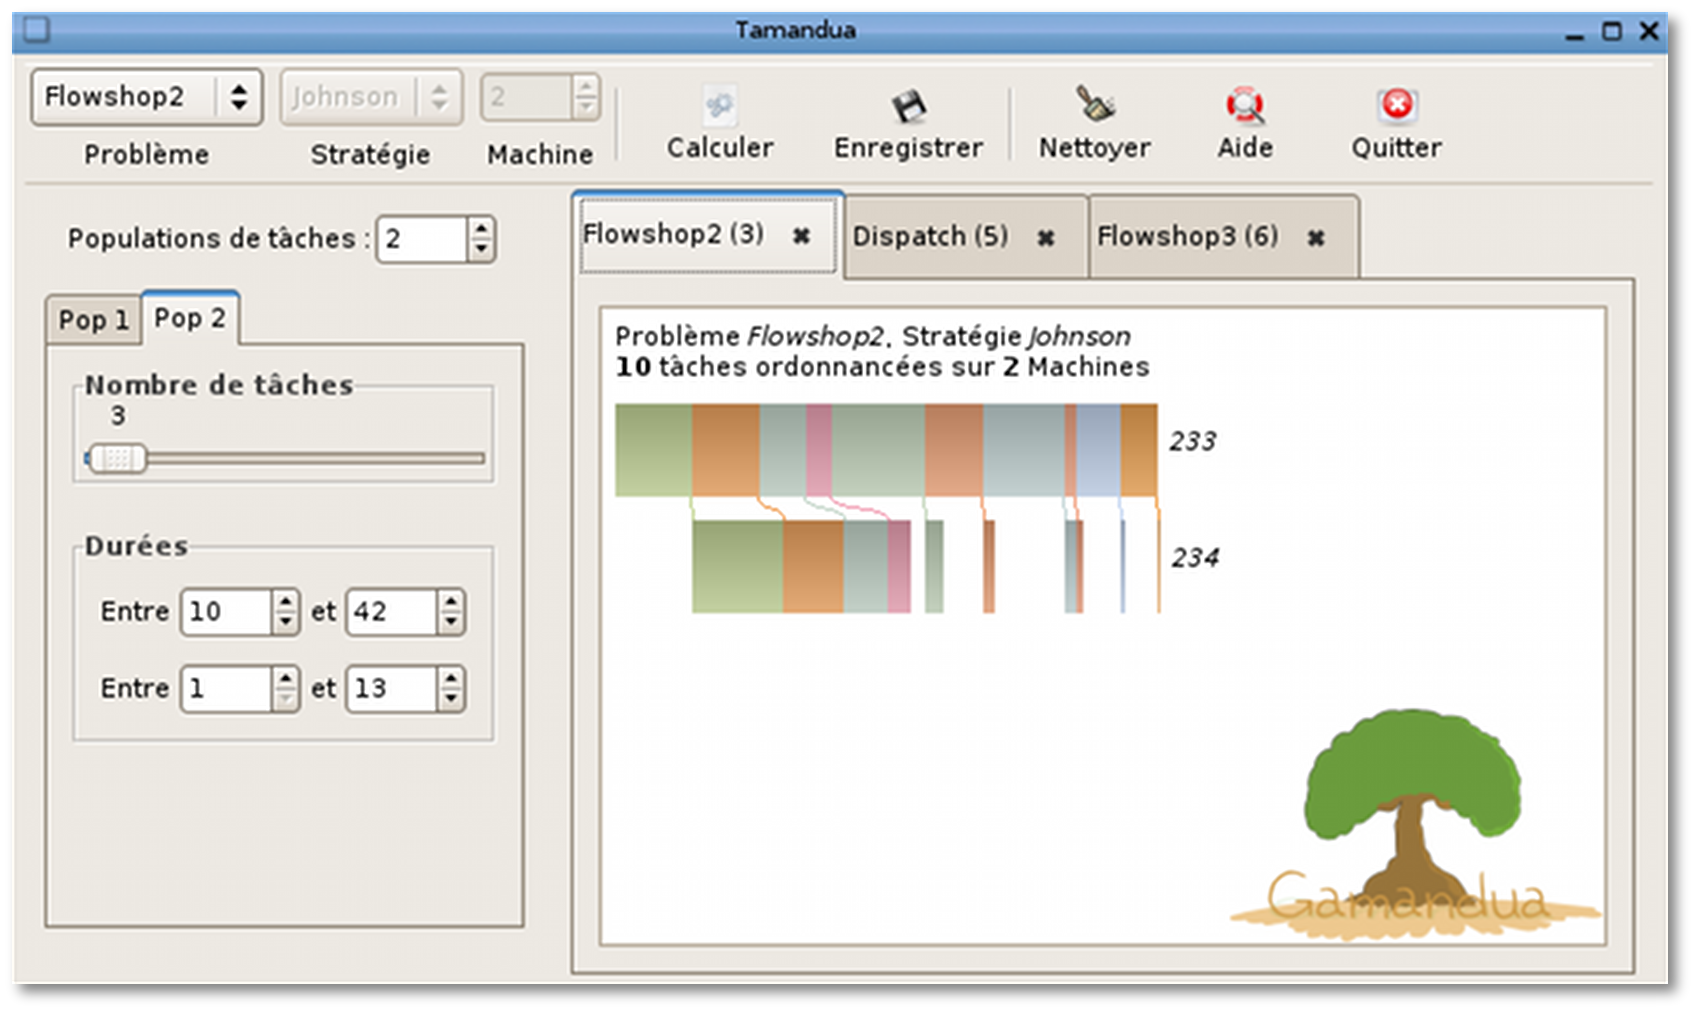
\includegraphics{gamandua.png}
\end{center}
Enfin le plus important au
milieu, les résultats des calculs, présentés sous forme de barres horizontales.
Dans le sens principal se trouve le temps, et à la verticale les différentes
machines, chaque tâche est représentée par un rectangle de couleur. La couleur
n'a aucune signification logique si ce n'est tenter de rendre le graphique
lisible. en cliquant sur les tâches une petite bulle s'affiche comportant des
informations supplémentaires. Plusieurs graphiques peuvent être conservés
simultanément grâce à un dispositif d'onglets en haut de l'affichage. Grâce au
bouton idoïne dans la barre d'outil, on peut exporter cette image en png si
on souhaite par exemple l'intégrer à un rapport ou la conserver en lieu sûr.
\subsection{Myrmidon}
Myrmidon est une interface réalisée en C++ grâce à la bibliothèque portable Qt.
Contrairement à Gamandua, elle est composée de plusieurs fenêtres, une fenêtre
principale affiche le résumé des simulations effectuées et permet d'ouvrir une
fenêtre de configuration de problèmes et de tâches. Chaque calcul se voit
ensuite attribué une fenêtre séparée afin de pouvoir les disposer librement et
de les afficher simultanément.

Afin de faciliter la liaison entre C++ et C et de réduire le couplage entre
l'interface et le noyau, une classe wrapper sert d'adaptateur et expose
l'interface du noyau en employant les concepts objets.
\begin{center}
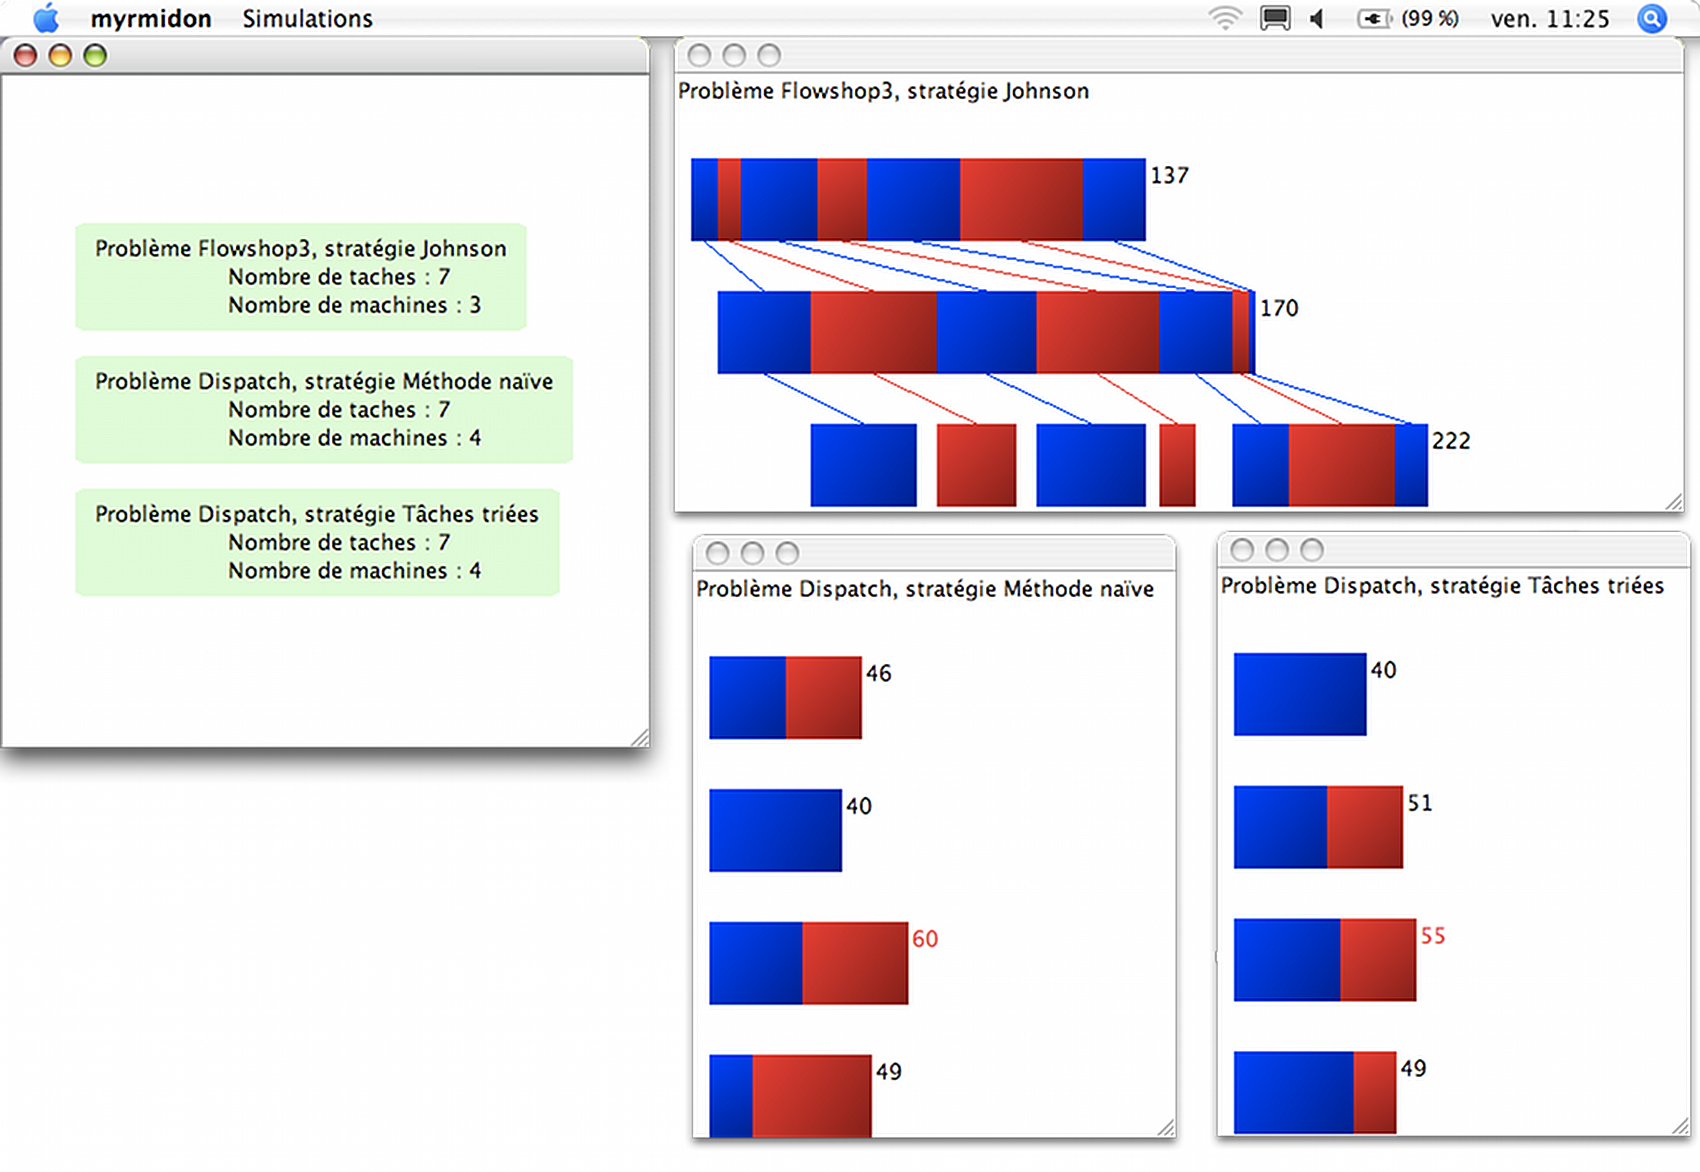
\includegraphics{myrmidon.png}
\end{center}
Un nouveau calcul se lance en cliquant sur Simulations $\rightarrow$ Nouvelle
Simulation dans le menu. Après configuration du calcul est validation, celui-ci
apparaît enfin. On note cependant qu'il n'est pas possible de gérer plus d'une
population dans la configuration.

Les fenêtres des calculs peuvent être fermées, puis réouvertes en cliquant sur leur résumé dans la fenêtre principale.

\end{document}
